\begin{frame}[allowframebreaks]{Fully Visible Sigmoid Belief Network (FVSBN)}
\textbf{Introduced by:} Bengio and Bengio (2000)

\textbf{Key Idea:}
\begin{itemize}
    \item A Bayesian network defined over observed variables, where each conditional distribution is modeled using a sigmoid (logistic) unit.
    \item All variables are visible; there are no latent or hidden variables in the model.
\end{itemize}

\textbf{Key Features:}
\begin{itemize}
    \item Each variable is conditionally independent of all others given its predecessors.
    \item The model captures complex dependencies between variables through a factorized representation.
    \item It allows for efficient computation of the joint probability distribution over the observed variables.
\end{itemize}

\framebreak

\textbf{Formulation:}
\begin{itemize}
    \item The joint probability of the vector $\mathbf{x} = (x_1, x_2, \ldots, x_n)$ is factorized as:
    \[
        p(\mathbf{x}) = \prod_{i=1}^n p(x_i \mid x_{<i})
    \]
    where $x_{<i} = (x_1, x_2, \ldots, x_{i-1})$.
    \item Each conditional is parameterized as:
    \[
        p(x_i = 1 \mid x_{<i}) = \sigma(W_i x_{<i} + b_i)
    \]
    where $W_i$ is a row vector of weights for the $i$-th variable, $b_i$ is a bias term, and $\sigma(z) = \frac{1}{1 + e^{-z}}$ is the sigmoid function.
\end{itemize}

\begin{figure}
    \centering
    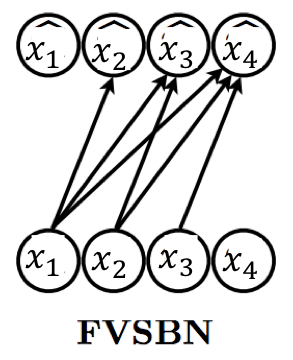
\includegraphics[height=1.0in]{images/arm/fvsbn.png}
    \caption{A fully visible sigmoid belief network over 4 variables}
\end{figure}

\framebreak

\begin{itemize}
    \setlength{\itemsep}{-0.25em}
    \item The conditional variables $X_i | X_1, X_2, \cdots X_{i-1}$ are Bernoulli with parameters
    \vspace{-1em}
    \begin{equation*}
        \hat{x}_i = \mathcal{P}(X_i=1 \mid x_1, \cdots, x_{i-1}; \alpha^i) = \mathcal{P}(X_i=1 \mid x_{<i}; \alpha^i) = \sigma (\alpha_0^i + \sum^{i-1}_{j=1}\alpha_j^i x_j)
    \end{equation*}
    \vspace{-1.5em}
    \item To evaluate $\mathcal{P}(x)$, we just multiply all the conditionals.
    \item To sample new images, we sample each $X_i$ chronologically.
    \begin{itemize}
        \item Sample $\overline{x}_1 \sim \mathcal{P}(x_1)$ np.random.choice([1,0], p=[$\hat{x}, 1-\hat{x}$])
        \item Sample $\overline{x}_2 \sim \mathcal{P}(x_2 | X_1=\overline{x}_1)$
        \item Sample $\overline{x}_3 \sim \mathcal{P}(x_3 | X_1=\overline{x}_1, X_2=\overline{x}_2)$
    \end{itemize}
    \item Total number of parameters = $1+2+3+ \cdots +n = \frac{n(n+1)}{2}$
    \item \textbf{Pros:} The likelihood is tractable and can be computed exactly.
    \item \textbf{Cons:} Poor scalability: each variable $x_i$ requires its own set of weights and bias, leading to a quadratic number of parameters as the number of variables increases.
\end{itemize}
\end{frame}


\begin{frame}{FVSBN: Results}

\begin{figure}
    \centering
    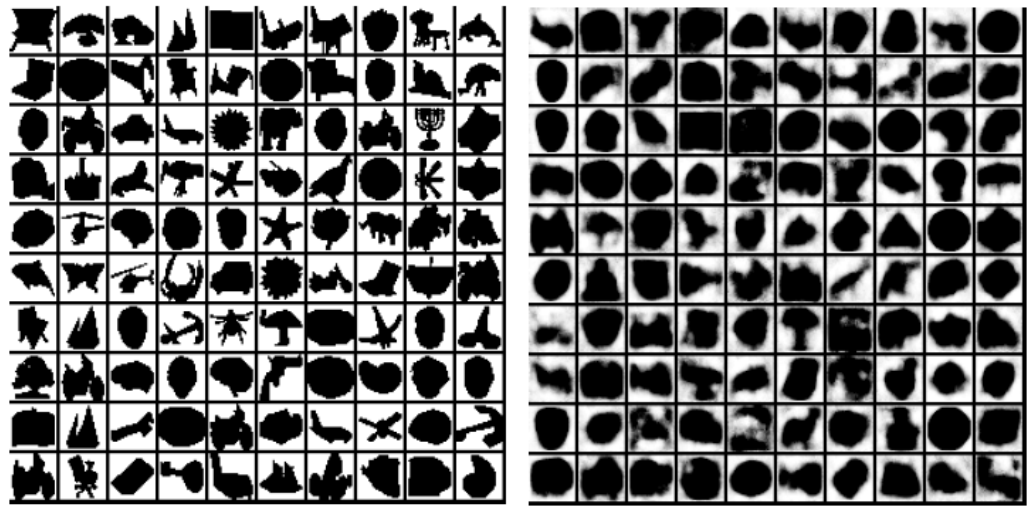
\includegraphics[height=2.0in]{images/arm/fvsbn_results.png}
    \caption{FVSBN results. Left: Training data. Right: Samples generated by model (Learning Deep Sigmoid Belief Networks with Data Augmentation, 2015)}
\end{figure}
    
\end{frame}